% PyBaMM Conference 2026 — 1-page abstract
% Submission requirements: A4, Arial >= 12pt, PDF, optional 1-2 figures
% Deadline: 2026-07-15 UTC
\documentclass[12pt,a4paper]{article}

% ── Arial-equivalent (Helvetica) as default face; venue requires Arial >= 12pt
\usepackage[T1]{fontenc}
\usepackage{helvet}
\renewcommand{\familydefault}{\sfdefault}

% ── Tight A4 margins to fit content on a single page
\usepackage[a4paper,top=1.8cm,bottom=1.8cm,left=1.8cm,right=1.8cm]{geometry}

\usepackage{graphicx}
\usepackage{caption}
\usepackage{subcaption}
\usepackage{microtype}
\usepackage{xcolor}
\usepackage[hidelinks]{hyperref}
\usepackage{setspace}
\setstretch{1.05}

\graphicspath{{../outputs/holdout_sweep/}}

% ── kill default title spacing
\usepackage{titling}
\setlength{\droptitle}{-2.2cm}

\pagestyle{empty}

\title{\vspace{-0.6cm}\textbf{\normalsize Physics-guided characterisation-time reduction for
second-life LFP cells:\\ how few cycles does PyBaMM's reaction-limited SEI need?}}
\author{\normalsize \textbf{\underline{Krishna Chaitanya Vaddepally}}$^{\dagger}$\\
  \small $^{\dagger}$Presenting author. Turno (Blubble Pvt.\ Ltd.), India.\\
  \small \texttt{battery.product@turno.club}}
\date{\vspace{-0.5cm}\small \textbf{Category:} Physics-based Models
      \quad $\bullet$ \quad \textbf{Preference:} Oral (poster acceptable)}

\begin{document}
\maketitle
\thispagestyle{empty}

\vspace{-1.0em}
\noindent\textbf{Motivation.}
Second-life repurposing of used lithium-iron-phosphate (LFP) cells for
stationary battery-energy-storage applications is bottlenecked by
characterisation cost: pack builders must estimate remaining useful life
(RUL) of cells for which no beginning-of-life data exists and for which
laboratory cycling time is limited. We ask a direct engineering
question: \emph{how many measured cycles does a physics-based degradation
model need before it can predict the remaining life of a used cell?}

\vspace{-0.3em}
\noindent\textbf{Method.}
We calibrate PyBaMM's reaction-limited SEI degradation model
(\texttt{Prada2013} chemistry, isothermal 25\,$^{\circ}$C) against the
measured fade slope of a used cell using only its first $K$ cycles, then
run the calibrated model to the full measured horizon and score against
the held-out cycles $K$--$N$. A single scalar (SEI exchange current density
$j_{\text{SEI}}$) is fit per cell by bisection on
$\log_{10}(j_{\text{SEI}})$; per-cell open-circuit voltage, initial
state-of-health, and ohmic resistance are constrained from HPPC and
OCV--SoC characterisation. We sweep $K \in \{50, 100, 200, 400, 800\}$
across seven MFR\_A-cohort cells with clean long-trajectory records
($N > 1000$ cycles each) that pass an upstream reaction-limited-shape
filter.

\vspace{-0.3em}
\noindent\textbf{Result.}
Prediction RMSE on held-out cycles drops from a median of 11.2\,pp SoH at
$K=50$ to $1.4$\,pp at $K=100$ and $0.5$\,pp at $K=800$ (Fig.~\ref{fig:rmse}).
At $K=400$ all 7/7 cells achieve
$\text{RMSE}_{\text{test}} < 3$\,pp SoH --- a $65$--$75\%$ reduction in
required cycling time versus full-trajectory calibration. Five of seven
cells already converge at $K=100$ with end-of-trajectory error below
$0.4$\,pp (Fig.~\ref{fig:cell07}). The remaining two exhibit a
post-formation recovery transient (positive apparent fade slope across
cycles 50--200) and require $K \geq 400$; this signal itself classifies
cells for correct calibration windowing.

% ── Figures side by side
\vspace{-0.3em}
\begin{figure}[h!]
  \centering
  \begin{subfigure}[t]{0.48\textwidth}
    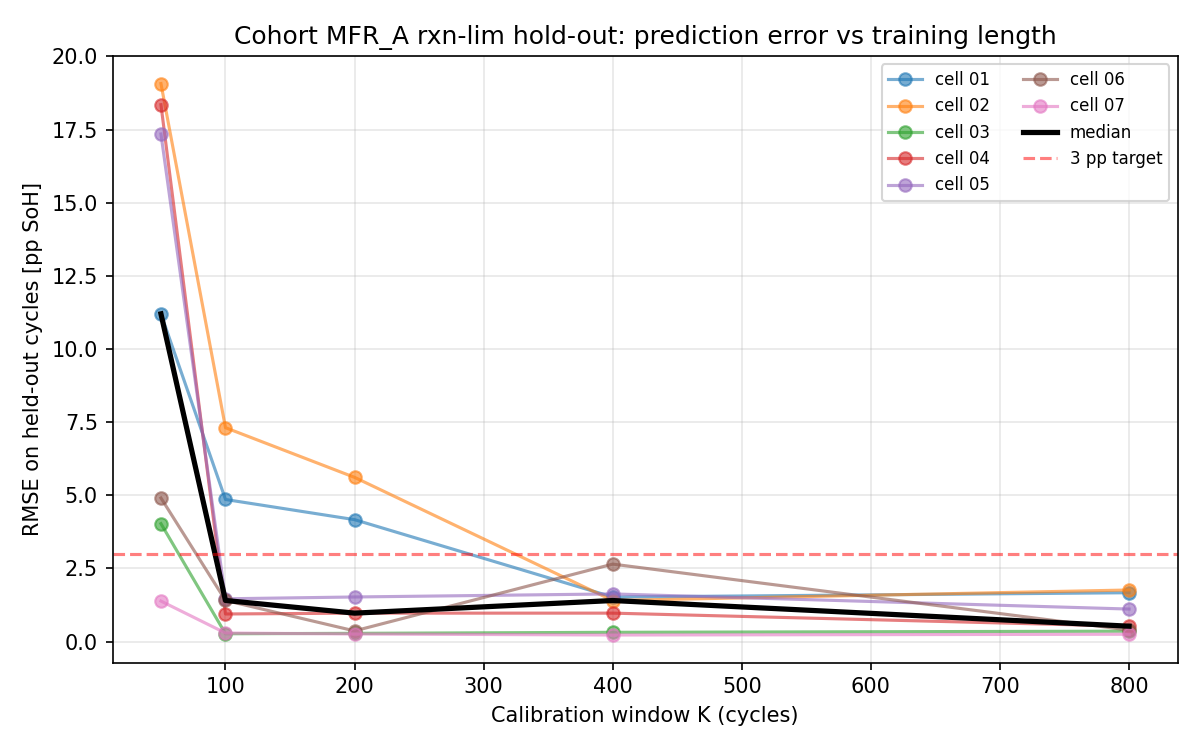
\includegraphics[width=\linewidth]{holdout_rmse_vs_K.png}
    \caption{Held-out RMSE vs.\ training window $K$; red dashed = $3$\,pp
      target.}
    \label{fig:rmse}
  \end{subfigure}\hfill
  \begin{subfigure}[t]{0.48\textwidth}
    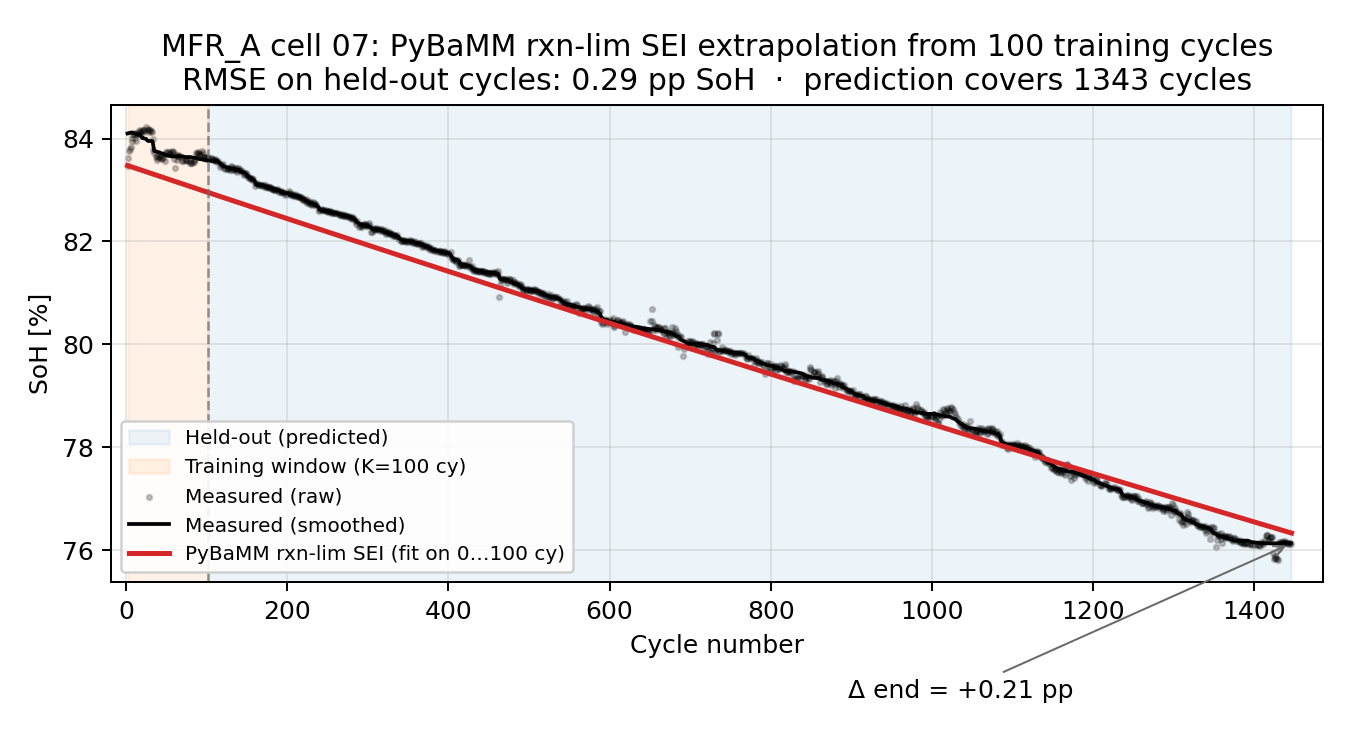
\includegraphics[width=\linewidth]{fig2_trajectory_cell_07.png}
    \caption{$K{=}100$-cycle fit predicts remaining $1345$ cycles of
      cell~07 to $0.29$\,pp SoH RMSE.}
    \label{fig:cell07}
  \end{subfigure}
\end{figure}

\vspace{-1.2em}
\noindent\textbf{Scope \& PyBaMM usage.}
The result holds only within the reaction-limited SEI regime; cells where
graphite loss-of-active-material dominates (identified upstream by
non-monotonic-early or three-regime shape) fall outside this envelope
because PyBaMM's stress-driven LAM formulation lacks saturation and
overfits short calibration windows. PyBaMM (\texttt{v26.4.3}) is the
calibration target and extrapolation engine; per-cell characterisation
is mapped into the \texttt{Prada2013} parameter set via
\texttt{build\_pybamm\_parameters}, and bisection over
$\log_{10}(j_{\text{SEI}})$ uses cached 10-cycle PyBaMM runs. Scripts
released at
\url{https://github.com/VKC-Turno/PyBaMM-Neural-ODE-RUL}.

\vspace{-0.6em}
{\small
\noindent\textbf{Acknowledgements.} The author thanks Sunil Kumar Rawat
(Imperial College London) for developing the initial cell parameter
identification and first-life PyBaMM degradation model on which this
work builds.\\[-0.3em]
\noindent\textbf{References.}
[1] V. Sulzer et al., \emph{J.\ Open Res.\ Softw.} 9(1) 14--21 (2021).
\;
[2] M. Prada et al., \emph{J.\ Electrochem.\ Soc.} 160(4) A616--A628 (2013).
}

\end{document}
